\documentclass[a4paper,12pt]{article}
\usepackage{graphicx}
\usepackage[left=30mm, right=30mm, top=30mm, bottom=35mm]{geometry}
\usepackage{amsmath}
\usepackage{siunitx}
\usepackage{fancyhdr}
\usepackage{booktabs}
\usepackage{url}
\usepackage{lscape}
\usepackage{cleveref}
\pagestyle{fancy}

%-------------------------------------------------------------------------------
\lhead{\textbf{Fall 2019}}
\rhead{\textbf{CE311K Intro to Computer Methods}}
\cfoot{\thepage}
%-------------------------------------------------------------------------------

\begin{document}
\begin{centering}
	\textbf{
		Project: Civil Engineering\\
		Assigned: 29th October 2019\\
		Partial code deadline (Qs 1 - 4): 15th November 2019 at 5 PM\\
		Reports due: 1st December 2019 at 5 PM\\
		This is a group project ($ 1 < size \le 3$), please submit individual reports\\
	}
\end{centering}


\vspace{1em}

Note: Please upload your code as .py, and ipynb files and your report as a pdf to the Canvas page. Solve questions 1 - 4 (no report required) for partial code deadline.

\vspace{1em}
 
 The purpose of this project is to develop your pair programming and debugging skills. Develop a Python module called \verb|utcivil| in the file  \verb|utcivil.py| that solves the following civil engineering applications.
 
\begin{enumerate}
	% Geotechnical engineering
	\subsection*{Geotechnical engineering}
	\subsubsection*{Control flow}
	\item In geotechnical engineering, we use a standardized process to classify soils into four basic types: gravel, sand, silt, and clay. 
	Gravel and sand are coarse-grained materials, because the soil particles are large. Gravels and sands are further subdivided into ``clean'' and ``dirty'' materials based on the amount of smaller-grained particles (i.e., ``fines'') found in the soil. ``Clean'' soils have less than 12\% fines and ``dirty'' soils contain more than 12\% fines.  The sieve test measures the percentage of different particle sizes and is used to classify soils, with the sieve number indicating the size of the openings in the sieve ($\#200$ sieve has openings of 0.075 mm, $\#4$ sieve has openings of 4.75 mm).
	
	Silt and clay are fine-grained materials, because the soil particles are small.  Silts and clays are further subdivided based on the ``stickiness'' or plasticity of the soil. The Atterberg Limit tests evaluate the ``stickiness'' of the soil and specifically measure the liquid limit (LL, the water content associated with liquid behavior of the soil), the plastic limit (PL, the water content associated with stiff, plastic behavior), and the plasticity index (PI = LL - PL). Soils can be classified using the criteria provided in~\cref{table:soil}.
	
	Note that there are two criteria for percent passing the \#200 sieve, but they must be used separately. The coarse fraction retained on the \#4 sieve can be calculated as:
	
	\begin{equation*}
		CF = \frac{100\% - \% pass\#4}{100\% - \% pass\#200} \times 100 \quad(\%)
	\end{equation*}
	
	Write a function that classifies a given soil into one of the soil types in~\cref{table:soil}. The function should accept four arguments (\% passing the $\#200$ sieve, the \% passing the $\#4$ sieve, the liquid limit (LL), and the plastic limit (PL)) and return a string as the soil classification. Classify the soils given in~\cref{table:classify}. 	To help check if your computer program is running correctly, the first sample should be classified as ``Sand - clean''.
	

	
	\begin{table}[!h]
		\caption{Classify the following soils}
		\label{table:classify}
		\centering
		\begin{tabular}{lp{3cm}p{3cm}p{2cm}p{2cm}}
			\toprule
			\textbf{Soil} & \textbf{\% Passing Sieve $\#200$} & \textbf{\% Passing Sieve $\#4$} & \textbf{Liquid Limit (LL)} & \textbf{Plasticity Limit (PL)} \\
			\midrule
			Soil A & 4  & 85  & 0  & 0  \\
			Soil B & 94 & 100 & 62 & 21 \\
			Soil C & 29 & 61  & 0  & 0  \\
			Soil D & 69 & 99  & 42 & 22 \\
			Soil E & 52 & 83  & 28 & 23 \\
			\bottomrule
		\end{tabular}
	\end{table}

	
	\begin{landscape}
	\centering
	\vspace*{5em}
	\begin{table}[!h]
		\begin{tabular}{lp{3cm}p{3cm}p{3cm}p{2cm}l}
			\toprule
			\textbf{Soil Type}     & \textbf{\% Passing Sieve \#200} & \textbf{Coarse Fraction Retained on \#4 Sieve} & \textbf{\% Passing Sieve \#200} & \textbf{Liquid Limit (LL)} & \textbf{Plasticity Index (PI)} \\
			\midrule
			Gravel - clean         & $ \le 50 \%$                    & $ \ge 50 \%$                                   & $< 12 \%$                       & --                         & --                             \\
			Gravel - dirty         & $ \le 50 \%$                    & $ \ge 50 \%$                                   & $ \ge 12\%$                     & --                         & --                             \\
			Sand - clean           & $ \le 50 \%$                    & $ < 50 \%$                                     & $< 12 \%$                       & --                         & --                             \\
			Sand - dirty           & $ \le 50 \%$                    & $ < 50 \%$                                     & $ \ge 12\%$                     & --                         & --                             \\
			Silt - low plasticity  & $ > 50 \%$                      & --                                             &                                 & $\le 50$                   & $< 0.73 (LL-20)$               \\
			Silt - high plasticity & $ > 50 \%$                      & --                                             &                                 & \textgreater 50            & $< 0.73 (LL-20)$               \\
			Clay - low plasticity  & $ > 50 \%$                      & --                                             &                                 & $\le 50$                   & $\ge 0.73 (LL-20)$             \\
			Clay - high plasticity & $ > 50 \%$                      & --                                             &                                 & \textgreater 50            & $ \ge 0.73(LL-20)$\\
			\bottomrule            
		\end{tabular}
		\caption{Soil classification}
		\label{table:soil}
	\end{table}
	\end{landscape}

	% Fluid mechanics
	\subsection*{Fluid mechanics}
	\subsubsection*{Bisection method}
	\item A flat plate of mass $m$ falling freely in air with a velocity $v$ is subject to a downward gravitational force and an upward frictional drag force due to air. The drag force $F_D$ is given by the expression:
	
	\begin{equation*}
		F_D = \frac{0.3 v^2}{500 + (\ln v)^3} - 0.02 v.
	\end{equation*}
	Terminal velocity is reached when the drag force equals the gravitational force. $F = F_D - mg = 0$. Using the \textit{bisection method} write a function to calculate the terminal velocity. Compute for the specific case of $m = $~\SI{1}{\kilogram} and $g =$~\SI{9.8}{\meter\per\second\squared}. Assume reasonable initial guess for $v$ in \textit{m/s}. Use a default relative tolerance of $1.e-5$. Return an error message if the solution could not be calculated or the initial guess range is invalid. 
	
	\item The following figure shows a rectangular open channel of constant dimensions. Under uniform flow conditions the flow in the channel is given by Manning's equation
	
	\begin{equation}
	\label{eq:q}
	Q = \frac{1}{n}\sqrt{S} A R^{2/3}
	\end{equation}
	
	where $S$ is the slope of the channel, $A$ is the are of the channel, $R$ is the hydraulic radius of the channel (the radius of a circle with equal area), $n$ is Manning's roughness coefficient. For a rectangular channgel, the following relationships hold:
	
	\begin{equation}
	\label{eq:ar}
	A = By \qquad R = \frac{By}{B + 2 y}
	\end{equation}
	
	where $y$ is the depth of the water in the channel.
	
	\begin{figure}[!h]
		\centering
		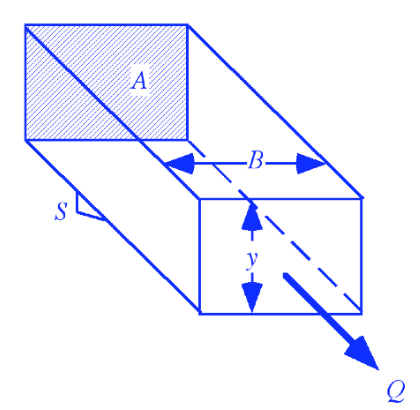
\includegraphics[width=0.3\textwidth]{figs/open-channel.png}
		\caption{Open channel flow}
	\end{figure}

	\textit{Substitute the relationships from~\cref{eq:ar} in~\cref{eq:q} and determine the non-linear equation to be solved. Write a function to compute the depth of water $y$ in the channel using the bisection method.}
	
	Using the following data: $Q = 14.15 m^3/s$, $B=4.572m$, $n = 0.017$, $S=0.0015$, using a suitable initial guess range of $1, 2$ solve for the depth of water in the channel. Use a default relative tolerance of $1.e-6$. Compute the number of iterations required to reach the solution.
	
	\item Write a generic bisection method function that takes the following arguments: the function to solve, exact solution, initial guess range, and a relative tolerance (set a default value of $1.e-6$). Using this bisection method function, rewrite the above functions, so as to not repeat the bisection code in the previous two fluid mechanics questions.
	
	\subsubsection*{Newton iterations}
	
	\item Infiltration is the process of water penetrating from the ground surface into soil. Depending on the amount of infiltration and the physical properties of the soil, water may penetrate a few centimeters to several meters into a soil. The cumulative infiltration is the accumulated depth of water infiltrated during a given time period.
	
	Using approximations of the governing equations of mass and momentum conservation for soil water, hydrologists have developed equations to estimate infiltration. One of the most commonly used infiltration equations is the Green-Ampt equation, which assumes that there is a
	sharp boundary dividing dry soil from saturated soil. The Green-Ampt equation for the cumulative infiltration of water into soil after a period of time is:
	
	\begin{equation}
		F = K t + \psi \delta\theta\ln\left(1 + \frac{F}{\psi\delta\theta}\right)
	\end{equation}
	
	where, 
	$F$ is the cumulative infiltration (cm), $K$ is the hydraulic conductivity of the soil (cm/hr), $t$ is the time (hr), $\psi$ is the suction head (cm), $\delta\theta\theta$ is the change in soil moisture content from the dry soil to the saturated soil. 
	
	Compute the cumulative infiltration after $1$ hour of infiltration into a soil that has the following characteristics: $K = 0.65 cm/hr$, $\psi = 16.7 cm$, $\delta\theta = 0.34$, and $t = 1 hr$.
	
	Write a function to solve the cumulative infiltration of water using the Green-Ampt equation. Use \textit{Newton's method} and start at an initial value of $F = Kt$. Derive the nonlinear function to solve. Compute the number of iterations to solve the nonlinear function with a tolerance of 1.e-5.
 	
 	\subsection*{Transportation engineering}
 	\subsubsection*{Taylor series}
 	\item A tranportation engineer involved in the evaluation of emission from vehicles uses an experimental system for studying the motion of a wide variety of cars in a full-scale laboratory environment. One particular test involves an accurate measurement of the displacement x of the vehicle as a function of time $t$. This information is then used to determine the velocity $v$ (first derivative), and acceleration $a$ (second derivative). In a given experiment, the displacement $x$ was measured over a time range of 0 - 10s, at steps of 1s. Some of the results obtained are given as follows:
 	
	\begin{table}[!h]
		\centering
 		\begin{tabular}{l c}
 			\toprule
 			\textbf{t (s)} & x(m) \\
 			\midrule
 			0 &	0 \\
 			1 &	3.5 \\
 			2 &	7.29 \\
 			3 &	11.45 \\
 			4 &	16.3 \\
 			5 &	21.1 \\
 			6 &	26.6 \\
 			7 &	39.5 \\
 			8 &	56.1 \\
 			9 &	75.1 \\
 			\bottomrule
 		\end{tabular}
		\caption{Vehicle distance data}
	 	\label{table:traffic}
	 \end{table}
 
 	Using the finite difference approximation of the first and second derivative estimate the velocity and acceleration of the car at 8s.
 	
 	\begin{align*}
 		f^\prime(a) & \approx \frac{f(a) - f(a - h)}{h} \\
 		f^{\prime\prime}(a) & \approx \frac{f(a + h) - 2 f(a) + f (a - h)}{h^2}
 	\end{align*}
 	
 	where $h$ is the interval. 
 	
 	Using the velocity and acceleration computed at 8s, compute how far the car moves at the end of 10s with a second-degree Taylor polynomial. Position at time $t$ is given by: $x(t) = \frac{1}{2}at^2 + v_0t + x_0$. 
 	
 	\begin{enumerate}
 		\item Develop the second-degree Taylor polynomial. 
 		\item Compute the distance traveled at the end of 10s.
 		\item Would it be reasonable to use this polynomial to estimate the distance traveled during the next minute? Explain.
 	\end{enumerate}
 

\end{enumerate}

\end{document}

